% \begin{frame}
% 	\frametitle{Wirkungsquerschnitt}
% 	\begin{figure}
% 	\begin{center}
% 	  \includegraphics[width=0.3\textwidth]{../img/atlas_higgs_event.png}
% 	  \caption{Produkte einer Proton-Proton-Kollision beim ATLAS-Experiment am CERN (Quelle: https://cds.cern.ch/record/1459496)}
% 	\end{center}
% 	\end{figure}
% 	\begin{itemize}
% 		\item Bei Streuprozessen ist der Endzustand nicht eindeutig bestimmt
% 		\item Der Wahrscheinlichkeit eines bestimmten Endzustandes wird durch den Wirkungsquerschnitt $\sigma$ beschrieben.
% 		\item Differentieller Wirkungsquerschnitt $\frac{\difd \sigma}{\difd O}$ in Bezug auf \\
% 			  Observable $O$ (z.B. Raumwinkel $\Omega$, Transversalimpuls $p_\text{T}, \ldots$)
% 	\end{itemize}
% \end{frame}

\section{Theoretische Grundlagen}

\subsection{Das Standardmodell}
 \begin{frame}
 	\frametitle{Das Standardmodell}
 	\begin{figure}
 	\begin{center}
 	  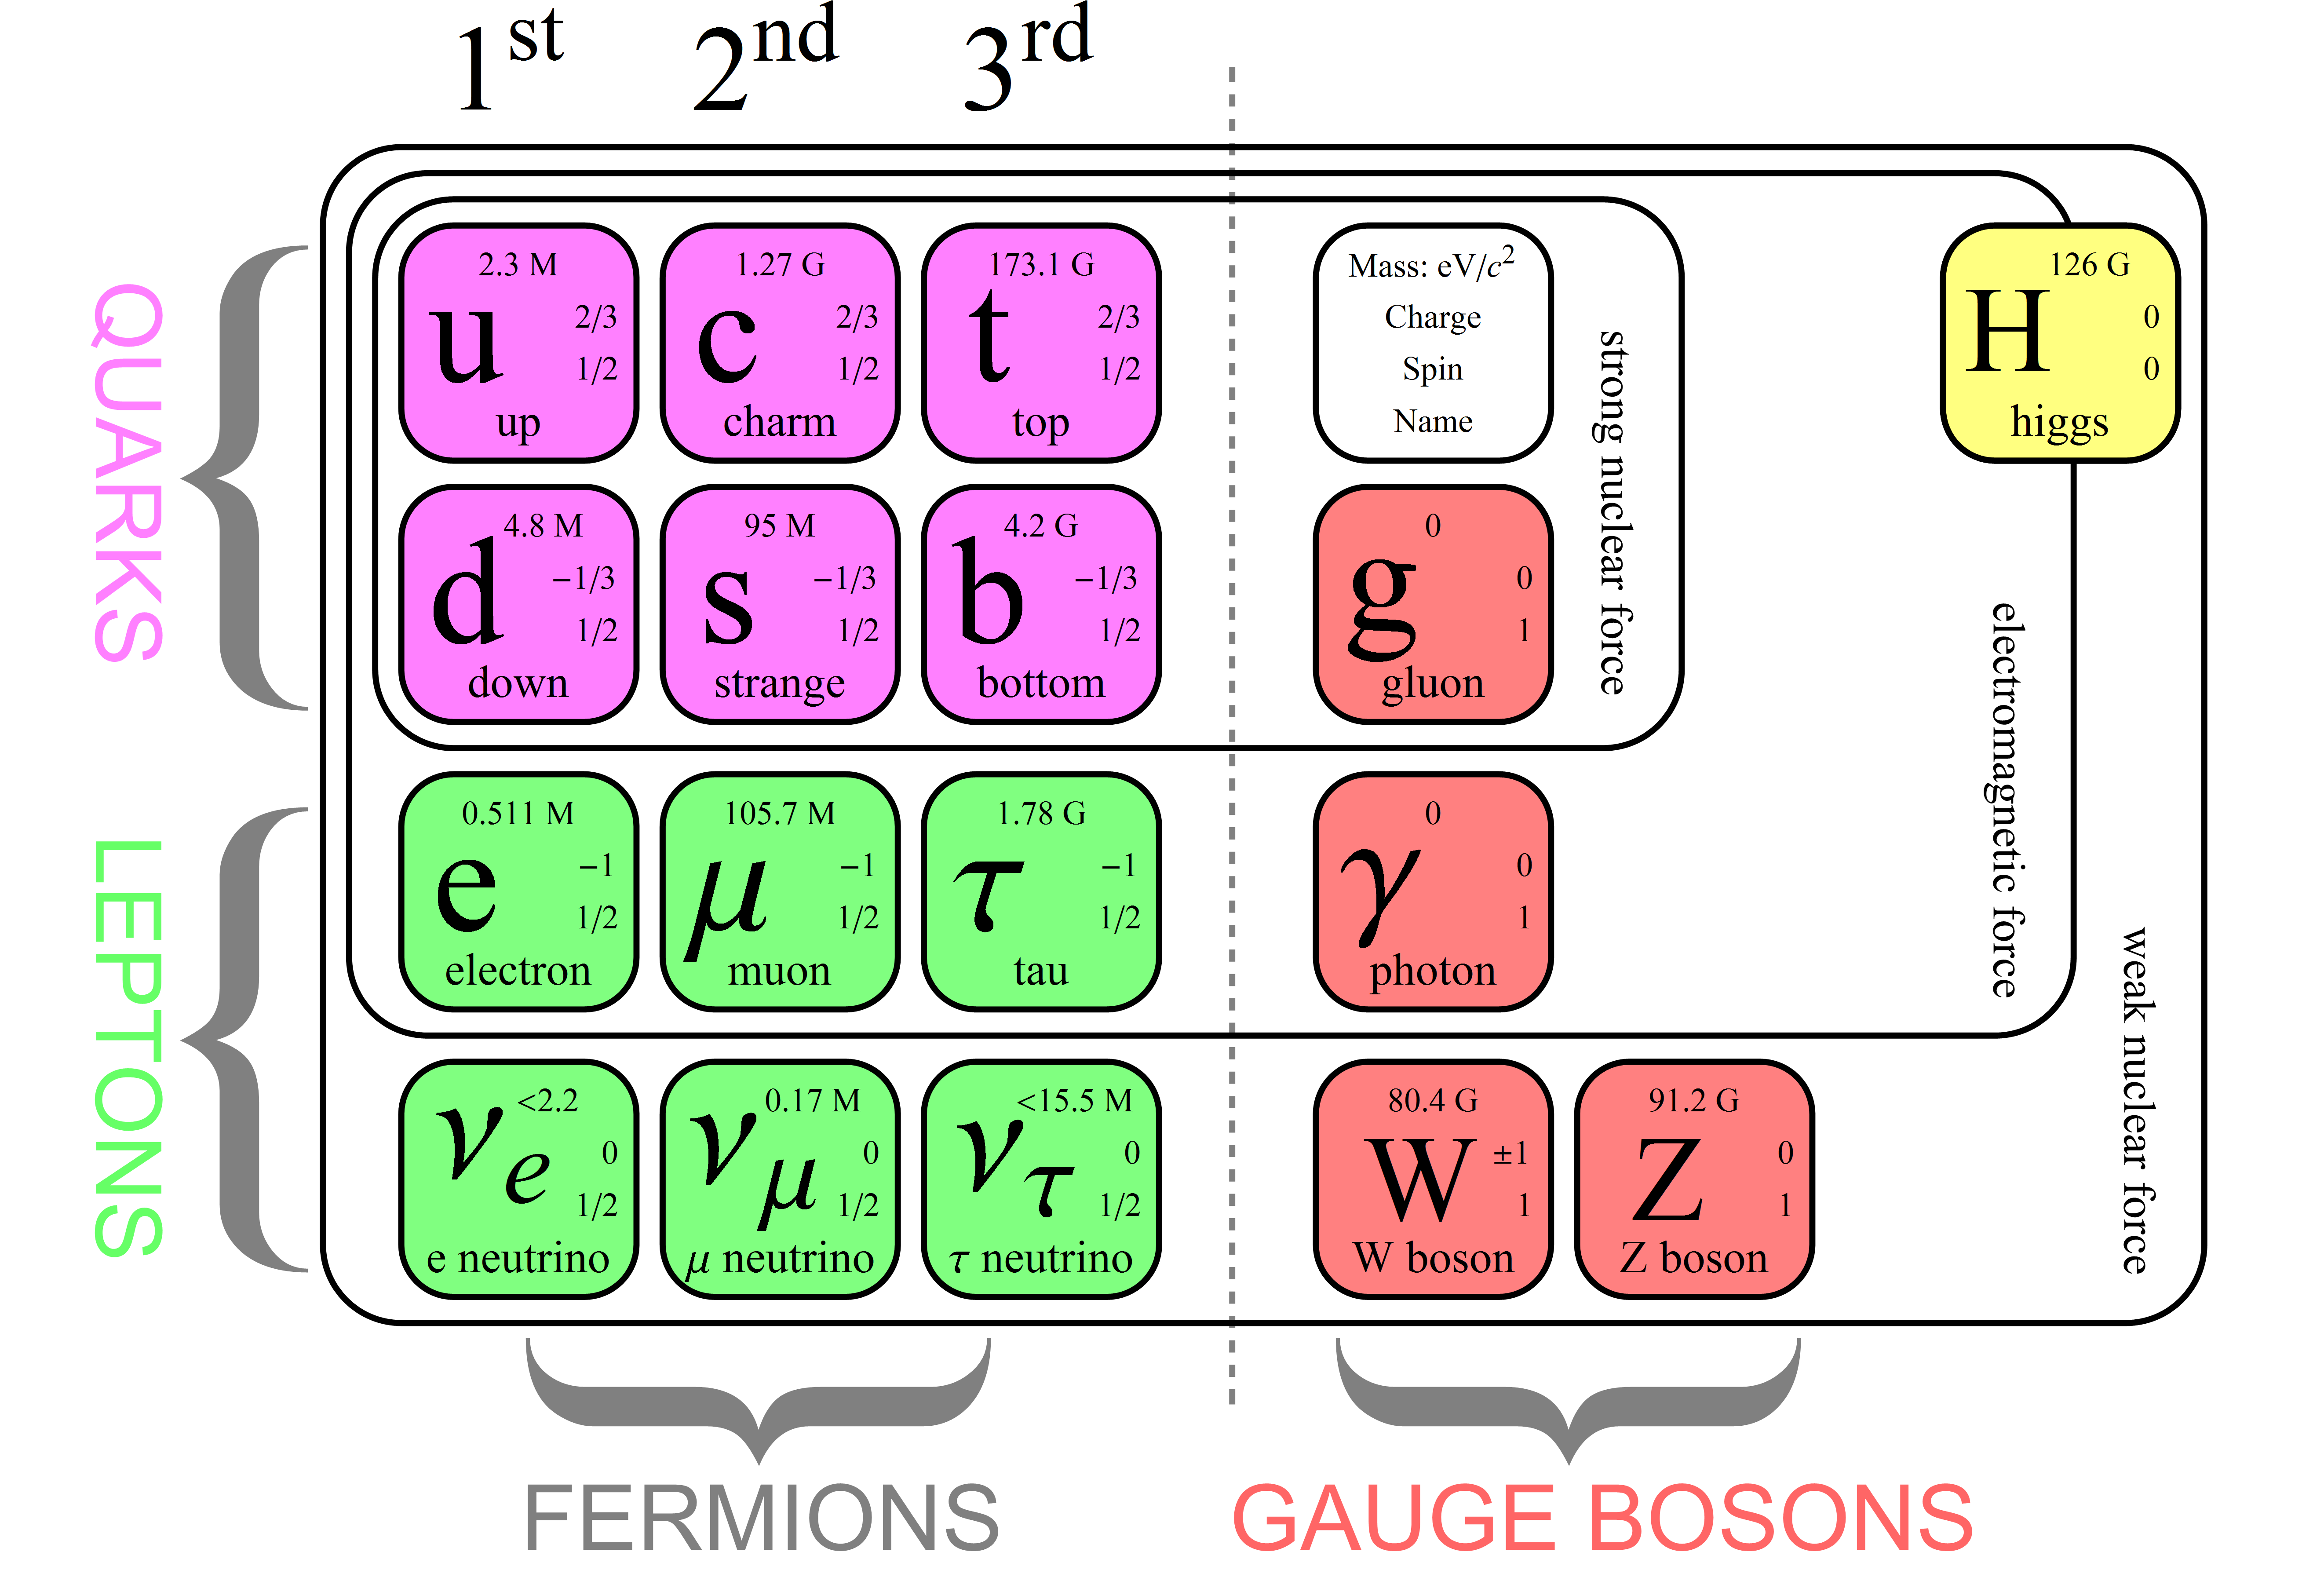
\includegraphics[width=0.9\textwidth]{graphics/SM1.png}
 	\end{center}
	\end{figure}
 \end{frame}
\begin{frame}
	\frametitle{Elektroschwache Wechselwirkung}
	\begin{center}
		\begin{itemize}
			\item
			Bei hohen Energien haben elektromagnetische und schwache WW ähnliche Kopplungsstärken.
			\item
			Vereinheitlichung der Theorien durch Glashow, Salam und Weinberg
			\item
			Einführung der Bosonen $W^1$, $W^2$, $W^3$, die am schwachen Isospin I koppeln und $B^0$, das an die schwache Hyperladung koppelt.
			\item
			Physikalische Zustände werden als Mischung dieser Bosonen beschrieben.
		\end{itemize}
		\begin{equation*}
		\begin{pmatrix}
		\ket{\gamma\;}\\
		\ket{Z^0}
		\end{pmatrix} = 
		\begin{pmatrix}
		cos(\theta_w) & sin(\theta_w)\\
		-sin(\theta_w) & cos(\theta_w)\\
		\end{pmatrix}
		\begin{pmatrix}
		\ket{B^0\:}\\
		\ket{W^3}
		\end{pmatrix}
		\end{equation*}
		\begin{equation*}
			\ket{\gamma} =  cos(\theta_w)\ket{B^0} + sin(\theta_w) \ket{W^3}
		\end{equation*}
		\begin{equation*}
		\ket{Z^0} = -sin(\theta_w) \ket{B^0} + cos(\theta_w) \ket{W^3}
		\end{equation*}
	\end{center}
\end{frame}

\begin{frame}
	\begin{center}
	\frametitle{Elektroschwache Wechselwirkung}
	Vektorkopplung (negativ bei Paritätstransformation)
	\begin{equation*}
	g_V^f = I^f_3-2 Q_f sin^2(\theta_w)
	\end{equation*}
	Axialvektorkopplung (postiv bei Paritätstransformation)
	\begin{equation*}
	g_A^f = I^f_3
	\end{equation*}
\end{center}
\end{frame}
\subsection{Wirkungsquerschnitt und Zerfallsbreite}
\begin{frame}
	\frametitle{Wirkungsquerschnitt}
	\hspace{1cm} Ereignisrate bei Luminosität $L$:
	\begin{equation*}
	\scalebox{1.5}{$\dot{N} = \sigma \cdot L$}
	\end{equation*}
	\hspace{1cm} Wirkungsquerschnitt messen:
	\begin{equation*}
	\scalebox{1.5}{$\sigma = \frac{N}{\int L~\text{d}t}$}
	\end{equation*}
\end{frame}
\subsection{$e^+e^-$ Kollisionen}
\begin{frame}
	\frametitle{Annihilation $e^+e^- \rightarrow f\bar{f}$ }
	\begin{center}
		\begin{figure}
			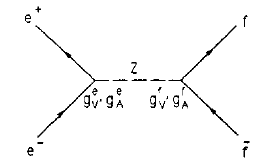
\includegraphics[width=0.5\textwidth]{graphics/presentationannihilation.png}
		\end{figure}
	\end{center}
	Untersuchte Prozesse:\\
	\begin{equation*}
	\begin{aligned}
	Z &\rightarrow e^+e^-\\
	Z &\rightarrow \mu^+\mu^-\\
	Z &\rightarrow \tau^+\tau^-\\
	Z &\rightarrow q\bar{q} \qquad\text{(außer top-Quark, da $M_{top} > M_Z$)}
	\end{aligned}
	\end{equation*}
	Nicht detektierbar:
	$Z \rightarrow \nu \bar\nu$
\end{frame}	
\begin{frame}
	\frametitle{theoretische Zerfallsbreiten der Prozesse}
	Unter Vernachlässigung der Fermionmassen gilt:
	\begin{equation*}	
	\Gamma_f=\frac{N_c^f \cdot \sqrt{2}}{12\pi}\cdot G_F \cdot M_Z^3 \cdot (g_V^{f2}+g_A^{f2})
	\end{equation*}
	\begin{table}[H]\centering
		\begin{tabular}{@{}llllll@{}}
			\toprule
			Fermion & $\Gamma _f\text{/MeV}$ \\
			\midrule
			e,$\mu $,$\tau $ & 83.4\\
			$\nu _e$,$\nu _{\mu }$,$\nu _{\tau }$ & 165.9\\
			u+d+c+s+b & 1741.7 \\
			\bottomrule
		\end{tabular}
	\end{table}
	Gesamtbreite:
	\begin{equation*}
	\Gamma_Z = \Gamma_e+ \Gamma_{\mu} + \Gamma_{\tau}+\Gamma_q + 3 \cdot \Gamma_{\nu}= 2489.6 GeV
	\end{equation*}
\end{frame}
\begin{frame}
	\frametitle{Schwerpunktsenergie und Wirkungsquerschnitt}
	\begin{equation*}
	\sigma(s) = \frac{12\pi}{ \tikzmark{MZ1}M_Z^2}
	\frac{s\tikzmark{gammae}\Gamma_e \tikzmark{gammaf}\Gamma_f}{(s-\tikzmark{MZ2}M_Z^2)^2 + s^2\cdot\tikzmark{gammaZ}\Gamma_Z^2 / \tikzmark{MZ3}M_Z^2}
	\end{equation*}
	%	\begin{tikzpicture}[
	%	remember picture,
	%	overlay,
	%	expl1/.style={draw=orange,fill=orange!30,rounded corners},
	%	expl2/.style={draw=gray!20,fill=gray!10,rounded corners},
	%	arrow1/.style={red!80!black,ultra thick,->,>=latex},
	%	arrow2/.style={gray!20,ultra thick,->,>=latex}
	%	]
	%	\node[expl1, text width=4cm]
	%	(gammaeexpl)
	%	at (2,2cm)
	%	{\textcolor{black}{Zerfallsbreite Elektron (Eduktteilchen)}};
	%	\node[expl1, text width=4cm]
	%	(gammafexpl)
	%	at (10,2cm)
	%	{\textcolor{black}{Zerfallsbreite Fermion (Produktteilchen)}};
	%	\node[expl1]
	%	(MZexpl)
	%	at (1,-1cm)
	%	{Masse $Z^0$};
	%	\node[expl1]
	%	(gammaZexpl)
	%	at (9.8,-1cm)
	%	{\textcolor{black}{Gesamtzerfallsbreite $Z^0$}};
	%	\draw[arrow1]
	%	(gammafexpl.west) to[out=180,in=90] ([yshift=-8.2ex,xshift=1.5ex]{pic cs:gammaf});
	%	\draw[arrow1]
	%	(gammaeexpl.east) to[out=0,in=90] ([yshift=2ex,xshift=0.5ex]{pic cs:gammae});
	%	\draw[arrow1]
	%	(gammaZexpl.west) to[out=180,in=270] ([yshift=-10.5ex,xshift=0.5ex]{pic cs:gammaZ});
	%	\draw[arrow1]
	%	(MZexpl.east) to[out=0,in=270] ([yshift=-10.5ex,xshift=1ex]{pic cs:MZ1});
	%\draw[arrow1]
	%(MZexpl.east) to[out=0,in=270] ([yshift=-10.5ex,xshift=1ex]{pic cs:MZ2});
	%\draw[arrow1]
	%(MZexpl.east) to[out=0,in=270] ([yshift=-10.5ex,xshift=1ex]{pic cs:MZ3});
	%	\end{tikzpicture}
	\begin{figure}
		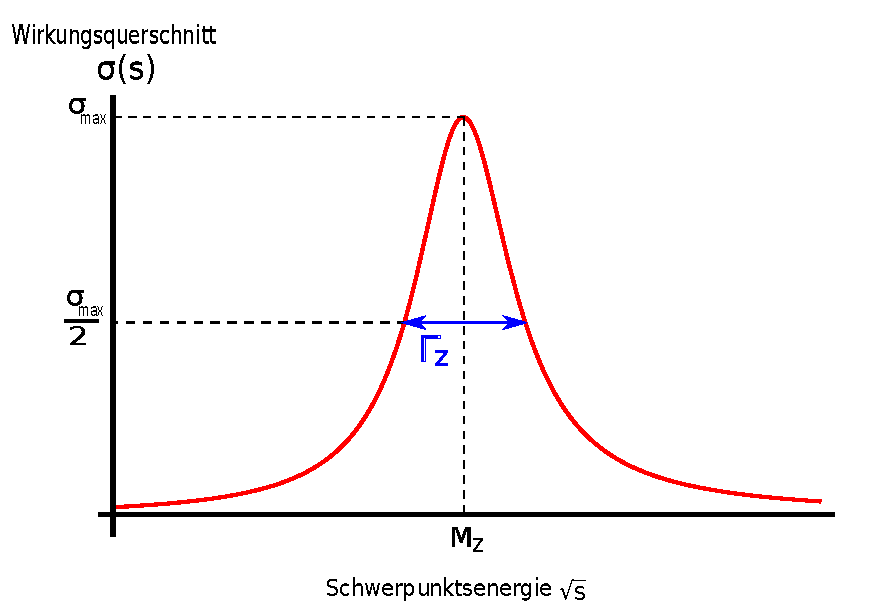
\includegraphics[width=0.75\linewidth]{graphics/Breit-Wigner}
	\end{figure}
\end{frame}
\begin{frame}
	\frametitle{ $e^+e^- \rightarrow e^+e^-$ s- und t- Kanal}
		\begin{minipage}{0.49\linewidth}
			\ \\
			\begin{figure}
				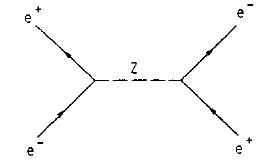
\includegraphics[width=1.1\textwidth]{graphics/annihilationee.png}
			\end{figure}
		\begin{equation*}
		\frac{d\sigma_s}{d\Omega} \propto (1+cos^2(\theta))
		\end{equation*}
	\end{minipage}
	\begin{minipage}{0.49\linewidth}
		\begin{figure}
			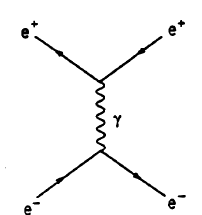
\includegraphics[width=0.8\textwidth]{graphics/BhabbaStreuungpresentation.png}
		\end{figure}
	\begin{equation*}
	\qquad\frac{d\sigma_t}{d\Omega} \propto (1-cos(\theta))^{-2}
	\end{equation*}
	\end{minipage}
\end{frame}
\begin{frame}
	\frametitle{Strahlungskorrekturen}
	\begin{figure}
		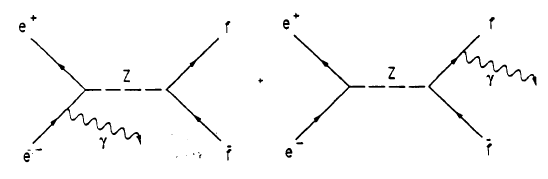
\includegraphics[width=0.75\linewidth]{graphics/Bremsstrahlungskorrektur}
	\end{figure}
	\begin{center}
	\begin{minipage}{0.4\linewidth}
			\begin{figure}
				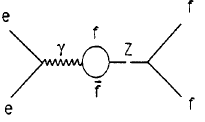
\includegraphics[width=0.8\linewidth]{graphics/presentationvertexschleifen}
			\end{figure}
	\end{minipage}
	\begin{minipage}{0.4\linewidth}
	\begin{figure}
			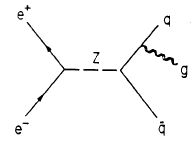
\includegraphics[width=0.8\linewidth]{graphics/presentation_QCDkorrektur}
	\end{figure}
	\end{minipage}
	\end{center}
\end{frame}

\subsection{Vorwärts Rückwärts Asymmetrie}
\begin{frame}
	\frametitle{Vorwärts Rückwärts Asymmetrie}
	\begin{figure}
		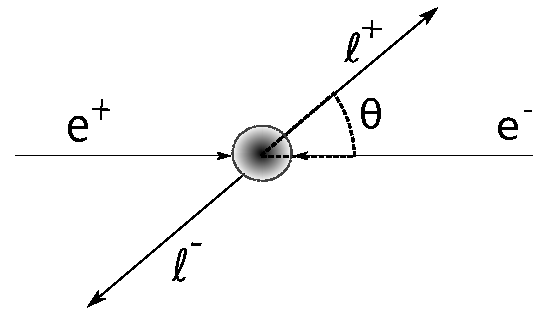
\includegraphics[width=0.3\textwidth]{graphics/AsymmetrieWinkel}
	\end{figure}

		Vordere Hemisphäre:
		\begin{equation*}
		\sigma_f=\int_{0}^{1}\frac{\text{d}\sigma}{\text{d}cos(\theta)}~\text{d}cos(\theta)
		\end{equation*}
		Hintere Hemisphäre:
		\begin{equation*}
		\sigma_b=\int_{-1}^{0}\frac{\text{d}\sigma}{\text{d}cos(\theta)}~\text{d}cos(\theta)
		\end{equation*}
		Asymmetrie:
		\begin{equation*}
		A_{fb}=\frac{\sigma_f-\sigma_b}{\sigma_f+\sigma_b}
		\end{equation*}
\end{frame}
\begin{frame}
	\frametitle{Vorwärts Rückwärts Asymmetrie}
		Für Leptonen am Resonanzpeak gilt:
		\begin{equation*}
		A_{fb}^{\ell,peak}\approx 3 \left ( \frac{g^{\ell}_V}{g^{\ell}_A} \right )^2=3\cdot (1-4 sin^2(\theta_w))^2
		\end{equation*}
		liefert Bestimmungsgleichung für elektroschwachen Mischungswinkel:
		\begin{equation*}
		\theta_w\approx\arcsin(\sqrt{\frac{1-\sqrt{A_{fb}/3}}{4}})
		\end{equation*}
\end{frame}